
In questa sezione verranno riportato il bilancio delle ore dei vari componenti del gruppo in base ai ruoli sostenuti. Il bilancio sarà così analizzato:
\begin{itemize}
	\item {\bfseries in positivo}: se il numero delle ore effettuate è minore rispetto a quelle preventivate;
	\item {\bfseries in negativo}: se il numero delle ore effettuate è maggiore rispetto a quelle preventivate;
	\item {\bfseries in pari}: se il numero delle ore effettuate è uguale rispetto a quelle preventivate; \\
\end{itemize}

\subsection {Analisi dei requisiti}
Verranno analizzate le ore di lavoro effettuate durante l'analisi dei requisiti, destinate principalmente allo studio personale; quindi non rendicontate.
\subsubsection{Prospetto orario}
	\begin{table} [h!]
	\begin{center}
		\rowcolors{2}{gray!25}{gray!6}
		\begin{tabular} { m{6 cm} c c c c c c c c }
			\rowcolor{lightgray}
			\textbf{Nome} & \textbf{Re} & \textbf{Am} & \textbf{An} & \textbf{Pg} &\textbf{Pr} & \textbf{Ve} & \textbf{Totale} \\ 
			Matteo Alba & 0 & 8(+1) &8(-2) & 0 & 0 & 10(+1) & 26  \\ 
			Giacomo Bulbarelli & 7 & 6(-1) & 8(+2) & 0 & 0 & 5(-1) & 26 \\ 
			Alessandro Chimetto & 7(-1) & 0 & 11(+2) & 0 & 0 & 8(-1) & 26 \\
			Alessandro Dindinelli & 0 & 4(-1) & 12(+1) & 0 & 0 & 10 & 26 \\
			Lucia Fenu & 0 & 6(-1) & 10(-2) & 0 & 0 & 10(+3) & 26 \\
			Paolo Scanferlato & 5(+1) & 7 & 6(-2) & 0 & 0 & 8(+1) & 26 \\
			Valton Tahiraj & 6(+1) & 5(-2) &7 & 0 & 0 & 8(+1) & 26 \\
			\textbf{Ore Totali Ruolo} & 25(+1) & 36(-4) & 62(-1) & 0 & 0 & 59(+4) & 182\\
		
		\end{tabular}
		\caption{Analisi dei requisiti - consuntivo ore/persona}
	\end{center}
\end{table}

	\begin{figure} [h!]
	\centering
	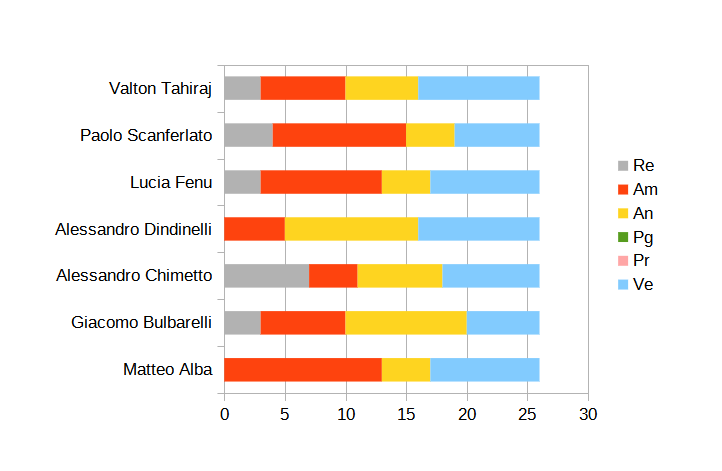
\includegraphics[width=0.7\textwidth]{res/img/grafici/consuntivo-barre_ ore analisi requisiti.png}
	\caption{Grafico consuntivo ruolo/ore - Analisi dei requisiti} 
\end{figure}


\newpage
\subsubsection{Prospetto economico}
Nella tabella sono riportate le ore totali per ciascun costo seguendo le indicazioni descritte all'inizio della sezione.
Allo stesso modo, il costo in euro sarà così analizzato:
\begin{itemize}
	\item {\bfseries in positivo}: la somma finale è minore rispetto a quella preventivata, il proponente ha risparmiato denaro;
	\item {\bfseries in negativo}: la somma finale è maggiore rispetto a quella preventivata, il proponente ha investito più denaro;
	\item {\bfseries in pari}: la somma finale è invariata rispetto a quanto preventivato. \\
\end{itemize}
\begin{table} [h!]
	\begin{center}
		\rowcolors{2}{gray!25}{gray!6}
		\begin{tabular} { m{3 cm} c c c  }
			\rowcolor{lightgray}
			\textbf{Ruolo} & \textbf{Ore} & \textbf{Costo in euro} \\
			Responsabile & 25(+1) & 750,00 (+120,00) \\
			Amministratore & 36(-4) & 720,00 (-80,00)  \\
			Analista & 62(-1) & 1550 (-25,00) \\
			Progettista & 0 & 0 \\
			Programmatore & 0 & 0  \\
			Verificatore & 59(+4) & 885,00 (+60,00)  \\
			\textbf{Totale} & 182  & 3905 (+75,00) \\
			
		\end{tabular}
		\caption{Prospetto economico - Analisi dei requisiti - Consuntivo}
	\end{center}
\end{table}

\begin{figure} [h!]
	\centering
	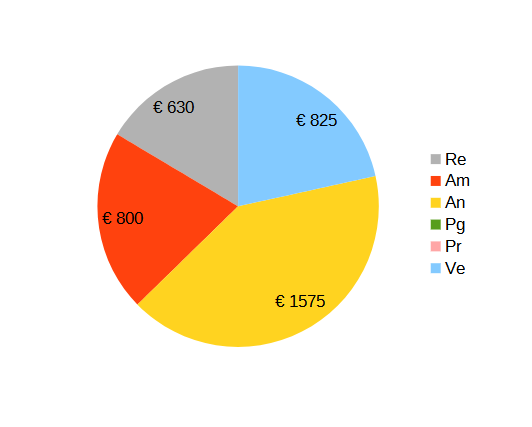
\includegraphics[width=0.6\textwidth]{res/img/grafici/consuntivo- torta_ costo_per_ora- analisi dei requisiti.png}
	\caption{Grafico consuntivo prospetto economico - Analisi dei requisiti} 
\end{figure}

\newpage 

\subsubsection{Conclusioni}
Il gruppo ha lavorato secondo le ore preventivate nel totale, anche se ci sono state delle correzioni all'interno dei ruoli dei singoli.
Nello specifico:
\begin{itemize}
	\item {\bfseries responsabile}: le ore previste, nel complesso, sono state rispettate;
	\item {\bfseries amministratore}: una maggiore attenzione nella gestione dei software e della documentazione, ha richiesto più tempo di quanto preventivato;
	\item {\bfseries analista}: le ore previste, nel complesso, sono state rispettate;
	\item {\bfseries verificatore}: grazie all'attenzione riposta nella gestione dei documenti, è stato svolto il ruolo di verificatore in meno ore rispetto alla previsione.\\
	
\end{itemize}

	\subsubsection{Preventivo a finire}
	A causa della variazione oraria di alcuni ruoli, il totale prevede una spesa inferiore di euro 75,00 rispetto a quanto preventivato.
	Tuttavia, la fase di analisi dei requisiti, non è rendicontata.
